% \mychapter{1}{Introduction}
\chapter{Introduction}

It is often the case in computational fluid dynamics that the velocity of the flow is not prescribed along all boundaries, and instead a natural boundary condition is used, where natural boundary conditions are those that are satisfied after a solution has been found. These boundary conditions can very often occur in practice and are particularly relevant in simulations of physiological flow such as blood moving through veins and arteries or air through the lungs \cite{bertoglio2017}, since in these cases the velocity of the flow on all boundaries can be hard to measure and rather the only available data is a combination of pressure and/or averaged flow. In general these biological systems being modelled may be exceptionally complex so in order to reduce the computational cost of finding a complete solution, the region of interest is usually truncated. Special care must then be taken to ensure the correct boundary conditions are prescribed along the boundaries of these truncated regions, especially where natural boundary conditions must be specified. Along these boundaries where natural boundary conditions occur, the biological systems discussed earlier may experience a reversal of flow due to periodicity in the physiology of the systems and the physical regularity of the structure. This situation of flow reversal is known as backflow.\\
\\
\begin{figure}[t]
\centering
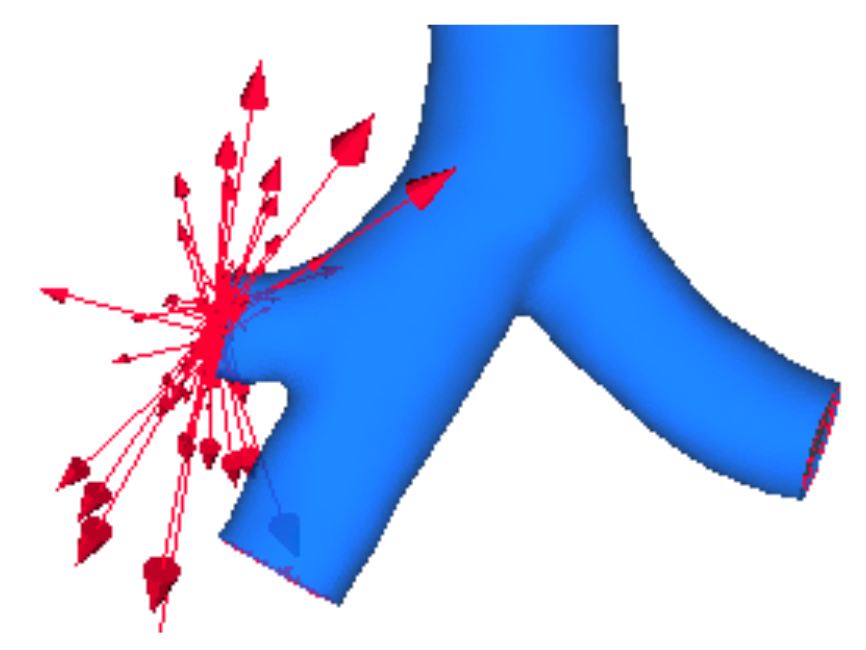
\includegraphics[width=5cm]{media/instability.PNG}
\caption{Numerical Instability when backflow occurs at an open boundary\label{fig:instab}}
\end{figure}

\section{Background}
The presence of backflow at open boundaries, boundaries where a natural boundary condition is prescribed, may cause the numerical simulation to become unstable. This can be seen graphically in figure \ref{fig:instab}. 
This instability is consistent in that in the presence of backflow there is a lack of general well-posedness results for the incompressible Navier-Stokes equations \cite[slide 24]{bertoglioLec01}: \begin{align}\label{NSeq}\begin{split}
 \rho\partial_t\textbf{u} + \rho(\textbf{u} - \textbf{w})\cdot\nabla\textbf{u} - 2\mu\nabla\cdot\epsilon(\textbf{u}) + \nabla p &= 0 \\ \nabla\cdot\textbf{u} &= 0 
 \end{split}\end{align}
 where \mathm{\rho} is the density, \textbf{u} is the background flow of the fluid, \textbf{w} is the flow of the domain, \mathm{\mu} is the viscosity, \mathm{\epsilon(\textbf{u})} is the strain rate tensor and \mathm{p} is the pressure. With some further constraints, these equations can then be rewritten into an energy balance as \cite[slide 11]{bertoglioLec12}:
 \begin{align}\label{NSeqENergy}
\partial_t\frac{\rho}{2}\int_{\Omega}\norm{\textbf{u}}^2 = -2\mu\int_{\Omega}\norm{\epsilon(\textbf{u})}^2 - \underbrace{\frac{\rho}{2}\int_{\Gamma_{N}}\textbf{u}\cdot\textbf{n}\norm{\textbf{u}}^2}_{(\text{\large \textasteriskcentered})}
 \end{align}
where \mathm{\Omega} is the entire domain and \mathm{\Gamma_{N}} is the boundary with the Neumann boundary condition. The term ({\large \textasteriskcentered}) has been particularly highlighted because it is this term which causes the instability when trying to solve (\ref{NSeq}) with open boundaries. It is this term that must be countered in order to obtain numerically stable solutions.\\
\\
Up to date, several proposals to overcome this issue have appeared in literature, mainly consisting in modifying the natural boundary conditions in order to enhance the overall stability \cite{bertoglio2017}. Two of these methods, velocity-penalization and velocity gradient penalization will be considered. The velocity-penalization method relies on counteracting the energy of ({\large \textasteriskcentered}) by modifying the natural boundary condition where backflow occurs with \cite[slide 15]{bertoglioLec12}:
\begin{align}\label{vp}
    2\mu\bm{\varepsilon} (\textbf{u})\textbf{n} - p{\bf n} ~{\color{red} + ~\beta\frac{\rho}{2}\abs{\bf\textbf{u}\cdot n}_{-}\textbf{u}} = {\bf g}_{N}, \qquad \beta \leq 1
\end{align}
This adjustment however has the issue that accuracy is affected by the extra term, especially since the outflow is perturbed by counteracting the backflow. Velocity gradient penalization method plays on the idea of rather stabilizing the local derivative of where the backflow occurs by adjusting (\ref{NSeqENergy}) with:  
\begin{align}\label{vgp}
\partial_t\frac{\rho}{2}\int_{\Omega}\norm{\textbf{u}}^2 = -2\mu\int_{\Omega}\norm{\varepsilon(\textbf{u})}^2 - \frac{\rho}{2}\int_{\Gamma_{N}}\textbf{u}\cdot\textbf{n}\norm{\textbf{u}}^2 ~{\color{red}- ~\frac{\rho}{2}\int_{\Gamma_{N}}\gamma\norm{{\bf t^{\text{T}}\nabla}\textbf{u}}^2}
\end{align}
This adjustment seems to have a lower accuracy impact as compared to the velocity-penalization method \cite{bertoglio2017}. 

\section{Problem Description}
The common trend among both these methods is that they both rely on a free parameter, \mathm{\beta} for the velocity-penalization method and \mathm{\gamma} for the velocity gradient method. There are values for both of these parameters for which stability has been proven, however it can also be seen experimentally that there are values for these parameters where the solution is stable and better accuracy is observed \cite{bertoglio2014}. Figures \ref{fig:velocompare} and \ref{fig:presscompare} show a comparison of both methods as well as how the solution can become more accurate when taking a different value for the parameter where stability is not guaranteed, and furthermore figure \ref{fig:flowcompare} shows how both methods compare when simulation the velocity profile on real geometry.\\
\begin{figure}[t]
\centering
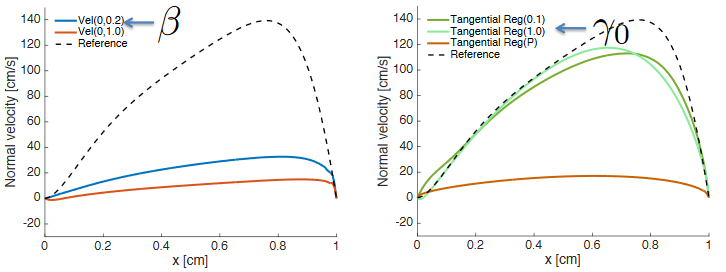
\includegraphics[width=12cm]{media/compare.PNG}
\caption{Comparison of the velocity-penalization and velocity gradient penalization when simulating a velocity profile\label{fig:velocompare}}
\end{figure}
\begin{figure}[t]
\centering
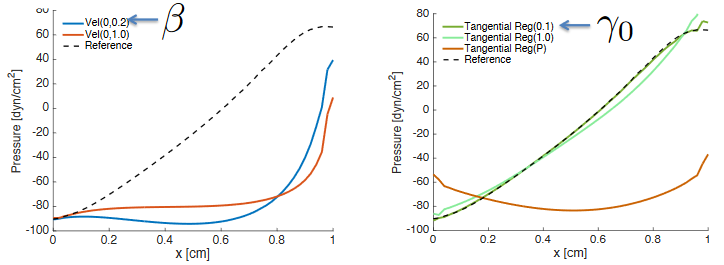
\includegraphics[width=12cm]{media/presscompare.PNG}
\caption{Comparison of the velocity-penalization and velocity gradient penalization when simulating a pressure profile\label{fig:presscompare}}
\end{figure}
\begin{figure}[t]
\centering
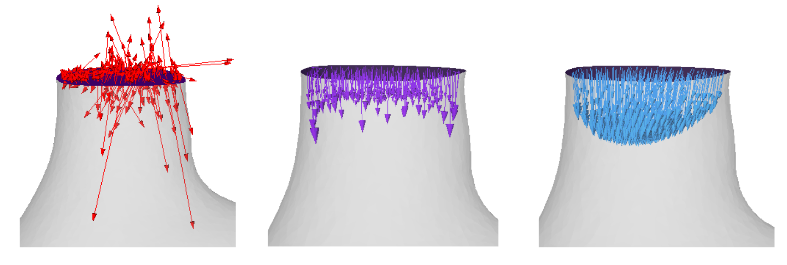
\includegraphics[width=12cm]{media/flowcomp.PNG}
\caption{Comparison of the velocity-penalization and velocity gradient penalization when simulating velocity on a real geometry\label{fig:flowcompare}}
\end{figure}
\\
Since the parameter must be chosen by the user before computation of the solution begins, the problem arises that if the parameter is chosen incorrectly, i.e. the solution becomes unstable, then the entire computation would have to be redone with a different parameter wasting all the previous computation time. How then should this parameter be chosen such that stability is maintained while improving the accuracy of the solution? Thus the focus in this paper will be to investigate how these two parameters can be chosen automatically during the computation such that stability is maintained while getting as accurate a solution as possible.\, which leads to the following research question: "Can these parameters be automatically chosen either at the beginning of- or during the computation such that we have optimum accuracy while maintaining stability of the solution".

\section{Possible solutions}

The approach that will be taken will be to transform \ref{vp} and \ref{vgp} into a weak form and then discretize them using a finite element method. We can analyse what effect the parameters have on the discretized problem, and then possibly we can determine on what a stable parameter depends, probably on the flow and pressure at the previous time step, as well as the other 'constants' such as viscosity and density. After this analysis has been completed we can then consider how to start the parameter selection.\\
\\
Possibilities include starting at the analytically guaranteed stable value and then slowly changing the value until, instability is detected, revert back to the last known stable value, refine the amount by which the value is changed and then repeat until a certain tolerance is reached. The problem with this method is that previous values of the  parameter must be stored, which would take up valuable space. A possibly better option may to still take a user-given input for the parameter but now it would be used as an initial guess, and then this value would be an initial value in a feedback loop of some type. The choice of which direction to pursue would be determined once the analysis described before has been completed.